\documentclass{atistandalonetask}
\usepackage{atistandard}
\begin{document}
  \begin{atiTask}[
    title = Die Ableitung der Delta-Distribution
  ]
    \begin{atiSubtasks}
    	\item Beweisen Sie durch vollständige Induktion, dass
    	\[
    	\integral{-\infty}{\infty}{f(x)\delta^{(n)}(x-x_0)}{x}=(-1)^nf^{(n)}(x_0)
    	\]
    	[$f^{(n)}$: $n$-te Ableitung von $f$]
    	\item Zeigen Sie durch Multiplikation mit einer Funktion $f(x)$ und Integration:
    	\[
    	x^m\delta^{(n)}(x)=\begin{cases}
    	0 & m>n\\
    	(-1)^n n!\delta(x)& m=n\\
    	\frac{(-1)^m n!}{(n-m)!}\delta^{n-m}(x) & m>n
    	\end{cases}
    	\]
    	\atiNote{\textsc{Leibniz}sche Produktregel:}
		\[
		\leibnizDerivative[n]{(uv)}{x}=\sum _{k=0}^n \frac{n!}{k! (n-k)!}\leibnizDerivative[k]{u}{x}\leibnizDerivative[n-k]{v}{x}
		\]
    \end{atiSubtasks}	
  \end{atiTask}
  \begin{atiSolution}
  	Lösung folgt
%  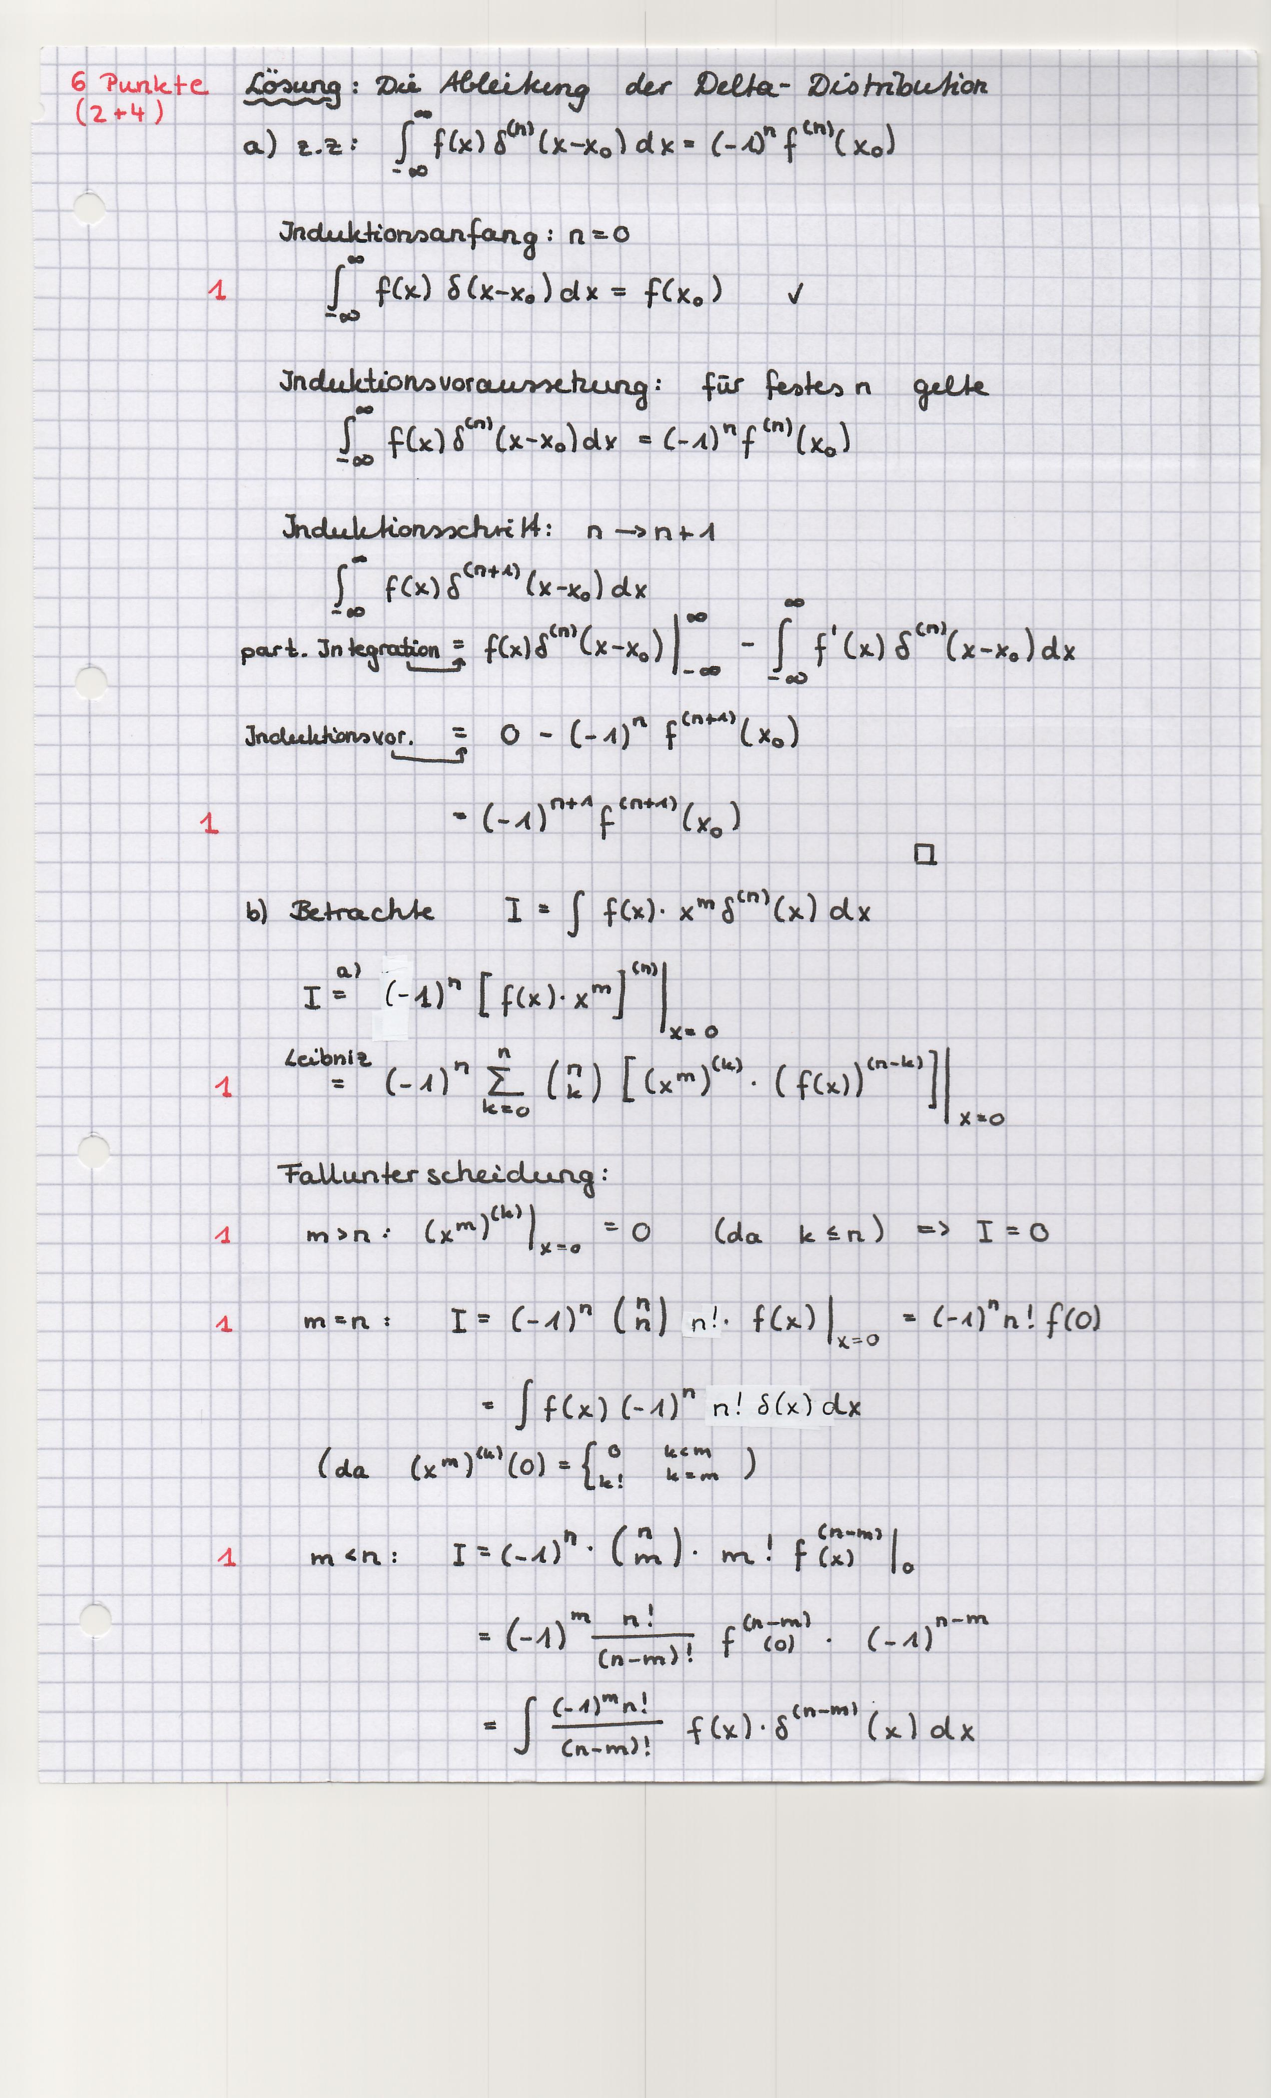
\includepdf[pages=-]{solution-delta_iv.pdf}
  \end{atiSolution}
\end{document}